\documentclass[11pt]{amsart}
\usepackage[margin=1.1in]{geometry}
\usepackage{amssymb,mathtools}
\usepackage{graphicx}
\graphicspath{{figures/}}
\usepackage[hidelinks]{hyperref}
\usepackage{doi}

\newcommand{\zenodoDOI}{10.5281/zenodo.XXXXXXXX}

\newtheorem{theorem}{Theorem}[section]
\newtheorem{lemma}[theorem]{Lemma}
\newtheorem{proposition}[theorem]{Proposition}
\newtheorem{corollary}[theorem]{Corollary}
\newtheorem*{theoremA}{Theorem A}
\newtheorem*{theoremB}{Theorem B}
\newtheorem*{propositionC}{Proposition C}
\theoremstyle{remark}
\newtheorem{remark}[theorem]{Remark}

\newcommand{\so}{\mathfrak{so}}
\newcommand{\h}{\mathfrak{h}}
\newcommand{\R}{\mathbb{R}}
\newcommand{\C}{\mathbb{C}}
\DeclareMathOperator{\Cl}{Cl}

\begin{document}

\title{Spinors of Exceptional Super Yang--Mills Theories Are Not Brane Cohomologies}

\author{Deep Bhattacharjee}
\address{Formerly, Electro-Gravitational Space Propulsion Laboratory (EGSPL), Bhubaneswar, Odisha 751030, India}
\address{Formerly, University of Calcutta (Heramba Chandra College), 23/49 Gariahat Road, Golpark, Kolkata 700029, West Bengal, India}
\email{d.bhattacharjee@erl-forschung.de}
\email{itsdeep@live.com}
\email{egspl@proton.me (GitHub-related contact; GitHub: creelie)}
\urladdr{https://orcid.org/0000-0003-0466-750X}

\subjclass[2020]{15A66, 17B10, 81T60, 83E30}
\keywords{Spinors, Clifford algebras, branes, Casimir operator, exceptional periodicity}

\begin{abstract}
Rios, Marrani and Chester identified the Majorana--Weyl spinors of their exceptional super Yang--Mills theories in $(8n+3)+3$ dimensions with the total cohomology of the largest brane. We prove that no such identification exists for any $n\ge 1$: on every spinor the Casimir operator of the brane rotation algebra takes one value that no exterior power attains. Their dual M-theory in $13+1$ dimensions does not arise from the reduction they describe either.
\end{abstract}

\maketitle

\section{Introduction}

Rios, Marrani and Chester proposed in \cite{RMC19} a family of supersymmetric Yang--Mills theories in the signatures $(9+8n)+1$, $(10+8n)+2$, $(11+8n)+3$ and $(12+8n)+4$, which they called exceptional, by moving $4n$ timelike directions of Nishino's signatures \cite{Nis98} into space; supersymmetry in these dimensions goes back to \cite{Nis98,RSS98}. In \cite{RMC20} they took up the case $27+3$, in which the supersymmetry algebra
\begin{equation}\label{eq:algebra}
\{Q_\alpha,Q_\beta\}=(\gamma^{\mu\nu\rho})_{\alpha\beta}Z_{\mu\nu\rho}+(\gamma^{\mu_1\cdots\mu_7})_{\alpha\beta}Z_{\mu_1\cdots\mu_7}+(\gamma^{\mu_1\cdots\mu_{11}})_{\alpha\beta}Z_{\mu_1\cdots\mu_{11}}+(\gamma^{\mu_1\cdots\mu_{15}})_{\alpha\beta}Z_{\mu_1\cdots\mu_{15}}
\end{equation}
carries the charges of a $3$-, $7$-, $11$- and $15$-brane. That these theories cannot be built by repeating Nishino's construction is shown in \cite{Bha26}; related geometric questions for Yang--Mills fields and for compactifications are treated in \cite{BSB26,BFS26}. The present paper is about a different claim of \cite{RMC20}, made in its Section~III and intended to extend the observation of Dijkgraaf, Verlinde and Verlinde \cite{DVV97} that the sixteen central charges of the five-brane are fluxes through its homology cycles.

The claim reads as follows. Write $\Lambda^k\mathbf{15}$ for the $k$-th exterior power of the vector representation of $\so_{15}$. Equations (3.4) and (3.5) of \cite{RMC20} state that
\begin{equation}\label{eq:claim}
\underbrace{\mathbf{16384}}_{\so_{27,3}\text{ MW spinor}}=\bigoplus_{i}\Lambda^{2i+1}\mathbf{15},\qquad
\underbrace{\mathbf{16384}'}_{\so_{27,3}\text{ MW conj.\ spinor}}=\bigoplus_{i}\Lambda^{2i}\mathbf{15},
\end{equation}
covariantly under $\so_{15}$, and call the right-hand sides the odd and even cohomology of the $15$-brane, the largest brane in \eqref{eq:algebra}. The text before (3.4) says that the semispinor $\mathbf{32768}$ of $\so_{28,4}$ is the total cohomology of the same brane, and (3.6)--(3.8) assert, as ``a general fact'', that for every level $n$ the semispinor $\mathbf{2}^{4n+3}$ of $\so_{8n+4,4}$ is the total cohomology of a $(4n+3)$-brane; for $n=1$ the $\mathbf{128}$ of $\mathfrak{e}_{8(-24)}$ is said to be the total cohomology of the $7$-brane.\footnote{The dimensions agree: $\sum_k\binom{15}{k}=2^{15}$ and $\sum_{k\ \mathrm{odd}}\binom{15}{k}=2^{14}$. The list printed in (3.5) of \cite{RMC20} ends in $\mathbf{25}'$, which should be $\binom{15}{14}=15$; with $25$ the list adds up to $16394$.}

Dimension counts cannot decide such a statement, since many modules share a dimension. The question is whether some subalgebra of $\so_{s,t}$ isomorphic to $\so_{4n+3}$ makes the spinor module isomorphic to a sum of exterior powers of its vector module. For the five-brane of \cite{DVV97} it does: there $\so_5\subset\mathfrak{gl}_5\subset\so_{5,5}$ acts on $\R^{5,5}=\R^5\oplus(\R^5)^*$, and the spinors of $\so_{5,5}$ restrict to $\Lambda^\bullet\R^5$ up to a power of the determinant \cite[\S 20.2]{FH91}. We show that in the signatures of \cite{RMC19,RMC20} it never does.

\begin{theoremA}
Let $n\ge 2$ and $m=4n+3$.
\begin{enumerate}
\item[(a)] Let $\h\subset\so_{8n+3,3}$ be a subalgebra isomorphic to a real form of $\so_m(\C)$. No exterior power of the vector module of $\h$ occurs in either semispinor of $\so_{8n+3,3}$, even after complexification.
\item[(b)] Let $\h\subset\so_{8n+4,4}$ be a subalgebra isomorphic to the compact algebra $\so_m$. No exterior power of the vector module of $\h$ occurs in either semispinor of $\so_{8n+4,4}$, even after complexification.
\end{enumerate}
\end{theoremA}

For $n=3$ this says that \eqref{eq:claim} is false for every choice of $\so_{15}$ inside $\so_{27,3}$, and that the $\mathbf{32768}$ of $\so_{28,4}$ is not the cohomology of a $15$-brane; for $n=2$ it says the same about $19+3$ and $20+4$. The case $n=1$ needs a separate argument, because $\so_7$ has an eight-dimensional spin module that fits into $\R^{12,4}$.

\begin{theoremB}
Let $\h$ be a subalgebra of $\so_{11,3}$ or of $\so_{12,4}$ isomorphic to the compact algebra $\so_7$. Neither semispinor contains $\Lambda^2\R^7$, $\Lambda^3\R^7$, $\Lambda^4\R^7$ or $\Lambda^5\R^7$, even after complexification. In particular the $\mathbf{128}$ of $\so_{12,4}$ is not $\Lambda^\bullet\R^7$ and the $\mathbf{64}$ of $\so_{11,3}$ is not $\bigoplus_i\Lambda^{2i+1}\R^7$.
\end{theoremB}

The obstruction is the signature. Over $\C$ the identification holds, through $\so_m(\C)\subset\mathfrak{gl}_m(\C)\subset\so_{2m}(\C)$, and Remark~\ref{rem:noncompact} shows that it also holds for the noncompact real form $\so_{4n+1,2}$ inside $\so_{8n+4,4}$; but the rotations of the spatial worldvolume of a brane form a compact algebra, and for $\so_{8n+3,3}$ no real form helps. The proofs rest on one computation, Lemma~\ref{lem:casimir}: on every spinor the Casimir operator of $\so_m$ equals $m(m-1)/8$, which is not an integer when $m\equiv 3\pmod 4$, while on $\Lambda^k$ it equals the integer $k(m-k)$ (Figure~\ref{fig:casimir}).

Section~II of \cite{RMC20} also introduces a ``dual M-theory'' in $13+1$ dimensions as the worldvolume theory of the magnetic dual of the $10$-brane, obtained by reduction from $26+2$ to $26+1$.

\begin{propositionC}
In the conventions of \cite{RMC20}, the reduction $26+2\to 26+1$ takes the $14$-brane with worldvolume $14+2$ to a $14$-brane with worldvolume $14+1$, not to the $13$-brane with worldvolume $13+1$; and the $10$-brane and the $14$-brane are not electric--magnetic duals in $26+1$ dimensions.
\end{propositionC}

Section~\ref{sec:prelim} fixes notation, Section~\ref{sec:small} bounds the small modules of $\so_{2l+1}$, Section~\ref{sec:embed} shows how such an algebra can sit in $\so_{s,t}$, Section~\ref{sec:proofs} proves Theorems~A and~B, and Section~\ref{sec:dual} proves Proposition~C. The finite arithmetic used below is rechecked by a short program in the archive of this paper \cite{Arch}; no proof depends on it.

\section{Preliminaries}\label{sec:prelim}

Let $V=\R^{s,t}$ with metric $\eta$ of signature $(s,t)$, and $V_\C=V\otimes\C$. The Clifford relations are $vw+wv=2\eta(v,w)$. When $s+t=2r$ the complex Clifford algebra $\Cl(V_\C)$ has a unique irreducible module $S$, of dimension $2^r$, and $S=S^+\oplus S^-$ under the chirality operator; $S^\pm$ are the semispinors. The Lie algebra $\so(V_\C)$ acts on $S$ through
\begin{equation}\label{eq:spinrep}
E_{v,w}\longmapsto \tfrac12\,vw\qquad(\eta(v,w)=0),
\end{equation}
where $E_{v,w}(x)=\eta(w,x)\,v-\eta(v,x)\,w$; indeed $\tfrac12(vwx-xvw)=\eta(w,x)v-\eta(v,x)w$ for $\eta(v,w)=0$ \cite[Ch.~I, \S 6]{LM89}. A Majorana--Weyl spinor of $\so_{s,t}$ is a real form of $S^+$ or $S^-$; it exists when $s-t\equiv 0\pmod 8$, as in all signatures considered here. A real $\so_{s,t}$-module and its complexification have the same submodule structure under any subalgebra up to complexification, so it suffices to prove Theorems~A and~B for $S^\pm$.

Let $U\subset V_\C$ be a nondegenerate subspace of dimension $m$ with a basis $u_1,\dots,u_m$ satisfying $\eta(u_i,u_j)=\delta_{ij}$. Write $E_{ij}=E_{u_i,u_j}$; these span $\so(U)$, which acts on $V_\C$ and is zero on $U^\perp$. The Casimir element
\begin{equation}\label{eq:casimir}
\Omega=-\sum_{1\le i<j\le m}E_{ij}^2
\end{equation}
is central in the enveloping algebra of $\so(U)$, so it acts by a scalar on every irreducible $\so(U)$-module and every module map between two modules intertwines it.

\begin{lemma}\label{lem:casimir}
\begin{enumerate}
\item[(i)] On $\Lambda^kU$ the element $\Omega$ acts by $k(m-k)$.
\item[(ii)] On $S$, and hence on $S^+$ and $S^-$, the element $\Omega$ acts by $m(m-1)/8$.
\item[(iii)] If $m\equiv 3\pmod 4$, then $m(m-1)/8\ne k(m-k)$ for every integer $k$.
\end{enumerate}
\end{lemma}

\begin{proof}
(i) We have $E_{ij}u_j=u_i$, $E_{ij}u_i=-u_j$ and $E_{ij}u_l=0$ for $l\notin\{i,j\}$, and $E_{ij}$ acts on $\Lambda^kU$ as a derivation. Let $u_I=u_{i_1}\wedge\dots\wedge u_{i_k}$ with $I=\{i_1<\dots<i_k\}$. If neither $i$ nor $j$ lies in $I$, then $E_{ij}u_I=0$. If both lie in $I$, then $E_{ij}u_I$ is a sum of two wedge products each containing a repeated vector, so it vanishes. If exactly one lies in $I$, then $E_{ij}$ exchanges $u_i$ and $u_j$ up to sign and $E_{ij}^2u_I=-u_I$. Exactly $k(m-k)$ pairs $\{i,j\}$ have one element in $I$, so $\Omega u_I=k(m-k)u_I$.

(ii) By \eqref{eq:spinrep}, $E_{ij}$ acts on $S$ as $\tfrac12u_iu_j$, and for $i\ne j$
\[
\bigl(\tfrac12u_iu_j\bigr)^2=\tfrac14u_iu_ju_iu_j=-\tfrac14u_i^2u_j^2=-\tfrac14 .
\]
Summing over the $\binom m2$ pairs gives $\Omega=\tfrac14\binom m2=m(m-1)/8$ on all of $S$.

(iii) If $m=4n+3$, then $m(m-1)/8=(4n+3)(2n+1)/4$, whose numerator is odd, so it is not an integer, while $k(m-k)$ is.
\end{proof}

\begin{figure}[t]
\centering
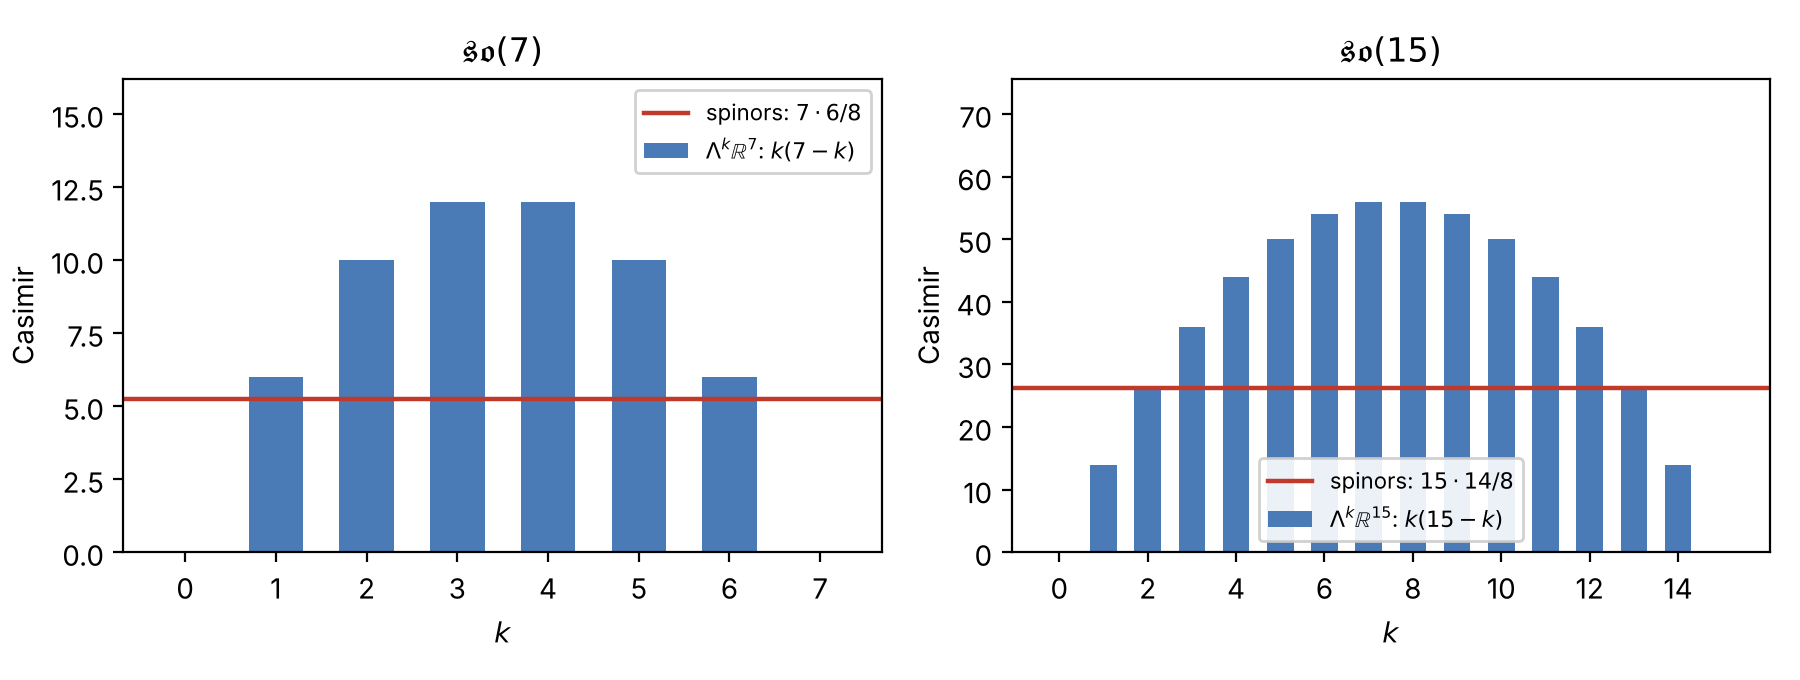
\includegraphics[width=\textwidth]{fig_casimir.png}
\caption{The Casimir operator \eqref{eq:casimir} on the exterior powers $\Lambda^k\R^m$ (bars) and on spinors (line), for $m=7$ and $m=15$. The line meets no bar.}
\label{fig:casimir}
\end{figure}

\section{Small modules of \texorpdfstring{$\so_{2l+1}$}{so(2l+1)}}\label{sec:small}

\begin{lemma}\label{lem:small}
Let $l\ge 3$ and let $W=\C^{2l+1}$ be the vector module of $\so_{2l+1}(\C)$. Every irreducible $\so_{2l+1}(\C)$-module of dimension less than $l(2l+1)$ is trivial, isomorphic to $W$, or isomorphic to the spin module, of dimension $2^l$.
\end{lemma}

\begin{proof}
Let $\omega_1,\dots,\omega_l$ be the fundamental weights, so that the irreducible module $V(\omega_i)$ is $\Lambda^iW$ for $i<l$ and $V(\omega_l)$ is the spin module \cite[\S 19.5]{FH91}. By the Weyl dimension formula,
\[
\dim V(\lambda)=\prod_{\alpha>0}\frac{(\lambda+\rho,\alpha)}{(\rho,\alpha)},
\]
and for dominant weights $\lambda,\mu$ each factor for $\lambda+\mu$ is at least the corresponding factor for $\lambda$, so $\dim V(\lambda+\mu)\ge\dim V(\lambda)$. Let $\lambda=\sum_ia_i\omega_i$ be dominant.

If $a_i\ge 1$ for some $2\le i\le l-1$, then $\dim V(\lambda)\ge\binom{2l+1}{i}\ge\binom{2l+1}{2}=l(2l+1)$, because the binomial coefficients increase up to $i=l$. Otherwise $\lambda=a\omega_1+b\omega_l$. If $a\ge 2$, then $\dim V(\lambda)\ge\dim V(2\omega_1)$, and $V(2\omega_1)$ is the traceless part of $\mathrm{Sym}^2W$, of dimension $(2l+1)(l+1)-1=l(2l+3)>l(2l+1)$. If $b\ge 2$, then $\dim V(\lambda)\ge\dim V(2\omega_l)=\dim\Lambda^lW=\binom{2l+1}{l}\ge l(2l+1)$. If $a\ge1$ and $b\ge1$, then $\dim V(\lambda)\ge\dim V(\omega_1+\omega_l)$, and $W\otimes V(\omega_l)=V(\omega_1+\omega_l)\oplus V(\omega_l)$ gives $\dim V(\omega_1+\omega_l)=2l\cdot 2^l\ge l(2l+1)$. The remaining weights are $0$, $\omega_1$ and $\omega_l$.
\end{proof}

\begin{corollary}\label{cor:small}
Let $m=4n+3$. If $n\ge 2$, every $\so_m(\C)$-module of dimension at most $8n+8$ is a sum of trivial modules and copies of $W$. If $n=1$, every $\so_7(\C)$-module of dimension at most $16$ is a sum of trivial modules, copies of $W=\C^7$ and copies of the spin module $\C^8$.
\end{corollary}

\begin{proof}
Here $l=2n+1$, and $8n+8<l(2l+1)=(2n+1)(4n+3)$ for all $n\ge1$. For $n\ge2$ also $8n+8<2^{2n+1}$: this holds for $n=2$ ($24<32$), and passing from $n$ to $n+1$ adds $8$ on the left and multiplies the right by $4$. For $n=1$, $16<21$. Finite-dimensional modules of $\so_m(\C)$ are completely reducible.
\end{proof}

\section{Embeddings of \texorpdfstring{$\so_m$}{so(m)} in \texorpdfstring{$\so_{s,t}$}{so(s,t)}}\label{sec:embed}

\begin{lemma}\label{lem:embed}
Let $\h\subset\so_{s,t}$ be a subalgebra isomorphic to a real form of $\so_m(\C)$, with $m$ odd, and let $V_0=\{v\in V:\h v=0\}$ and $V_1=\h V$. Then $V=V_1\oplus V_0$, the two summands are orthogonal and $\eta$ is nondegenerate on each.
\begin{enumerate}
\item[(a)] If $(s,t)=(8n+3,3)$, $m=4n+3$ and $n\ge2$, then $V_1\otimes\C$ is isomorphic to the vector module $W$ of $\h\otimes\C$.
\item[(b)] If $(s,t)=(8n+4,4)$, $m=4n+3$, $n\ge2$ and $\h$ is compact, then $V_1\otimes\C\cong W$ and $V_1$ is positive definite.
\item[(c)] If $(s,t)\in\{(11,3),(12,4)\}$ and $\h\cong\so_7$ is compact, then $V_1$ is positive definite of dimension $7$ or $8$, and $\h$ acts on it by the vector or the spin module.
\end{enumerate}
\end{lemma}

\begin{proof}
The module $V$ is completely reducible and $V_0$ is its isotypic component of trivial type, so $V=V_1\oplus V_0$. For $x\in V_0$, $X\in\h$ and $z\in V$ we have $\eta(x,Xz)=-\eta(Xx,z)=0$, so $V_0\perp V_1$, and since $\eta$ is nondegenerate on $V$ it is nondegenerate on both summands. The algebra $\so_{s,t}$ acts faithfully on $V$, hence so does $\h$, and $V_1\ne0$.

Every real form of $\so_m(\C)$ with $m$ odd is some $\so_{p,q}$ with $p+q=m$, and its vector module $\R^{p,q}$ is absolutely irreducible and carries an invariant form $b$ of signature $(p,q)$, unique up to a factor. If $V_1\otimes\C\cong W\oplus W$, then $V_1\cong\R^{p,q}\otimes\R^2$, and every invariant symmetric form on it is $b\otimes M$ with $M$ a symmetric $2\times2$ matrix, nondegenerate here. Diagonalising $M$ shows that the signature of $V_1$ is $(2p,2q)$, $(m,m)$ or $(2q,2p)$.

(a) By Corollary~\ref{cor:small}, $V_1\otimes\C$ is $W$ or $W\oplus W$. In the second case $V_1=V$ has dimension $2m=8n+6$ and signature $(8n+3,3)$; but $8n+3$ is odd, and $m>3$, so none of the three signatures above is possible.

(b) Now $p=m$, $q=0$. If $V_1\otimes\C\cong W\oplus W$, then $V_1$ has signature $(2m,0)$ or $(m,m)$ and $V_0$ has dimension $2$, so the number of negative directions of $V$ is at most $2$ or at least $m>4$, a contradiction. Hence $V_1\otimes\C\cong W$, and $b$ is definite; since $V_1$ has dimension $m>4$, it is positive definite.

(c) By Corollary~\ref{cor:small}, $V_1$ is a sum of copies of $\R^7$ and of the spin module $\R^8$, both carrying definite invariant forms unique up to a factor. The isotypic components are orthogonal, and as above an isotypic component with $c$ copies of a module of dimension $d$ has signature $(c'd,c''d)$ with $c'+c''=c$. With $d\in\{7,8\}$ and total dimension $14$ or $16$, the decompositions with at least two nontrivial summands are $\R^7\oplus\R^7$, $\R^7\oplus\R^8\oplus\R$ and $\R^8\oplus\R^8$, up to trivial summands; the numbers of negative directions of $V_1$ then lie in $\{0,7,14\}$, $\{0,7,8,15\}$ and $\{0,8,16\}$. Since $V_0$ has dimension at most $2$, the space $V$ would have at most $2$ or at least $7$ negative directions, never $3$ or $4$. So $V_1$ is one copy of $\R^7$ or of $\R^8$, definite, hence positive definite because $t<7$.
\end{proof}

\section{Proofs of Theorems A and B}\label{sec:proofs}

\begin{proof}[Proof of Theorem~A]
By Lemma~\ref{lem:embed}(a) or (b), $U=V_1\otimes\C$ is a nondegenerate subspace of $V_\C$ of dimension $m$ on which $\h\otimes\C$ acts by its vector module, and $\h$ is zero on $U^\perp=V_0\otimes\C$. Since $\h\otimes\C$ acts faithfully on $U$ and preserves $\eta$, and $\dim\h=\dim\so(U)$, the image of $\h\otimes\C$ in $\so(V_\C)$ is $\so(U)$, and the vector module of $\h$ is $U$. By Lemma~\ref{lem:casimir}(ii) the Casimir element of $\so(U)$ acts on $S^+$ and $S^-$ by $m(m-1)/8$, and by Lemma~\ref{lem:casimir}(i) it acts on $\Lambda^kU$ by $k(m-k)$. These numbers differ by Lemma~\ref{lem:casimir}(iii), so there is no nonzero $\h$-module map $\Lambda^kU\to S^\pm$.
\end{proof}

In the language of \cite{RMC20}: under any $\so_{15}$ inside $\so_{27,3}$ the module $\mathbf{16384}$ is $128$ copies of the spin module $\mathbf{128}$ of $\so_{15}$, and it contains none of the modules $\mathbf{15},\mathbf{455},\mathbf{3003},\mathbf{6435},\mathbf{5005},\mathbf{1365},\mathbf{105},\mathbf{1}$ of \eqref{eq:claim}. Indeed, choose a nondegenerate line $\ell\subset U^\perp$ and put $U'=U\oplus\ell$. Then $S\cong S_{U'}\otimes S_{U'^\perp}$ as a module over $\so(U')\oplus\so(U'^\perp)$, and both semispinors of $\so(U')\cong\so_{16}(\C)$ restrict to the spin module of $\so(U)\cong\so_{15}(\C)$, so $\so(U)$ acts on $S$ through copies of its spin module.

\begin{proof}[Proof of Theorem~B]
By Lemma~\ref{lem:embed}(c) there are two cases.

If $V_1\cong\R^7$, the argument of Theorem~A applies with $m=7$: the Casimir element acts by $21/4$ on $S^\pm$ and by an integer on every $\Lambda^k\R^7$.

If $V_1\cong\R^8$ with $\h$ acting by the spin module, let $U=V_1\otimes\C$. Then $\h\otimes\C$ lies in $\so(U)\cong\so_8(\C)$ as the image of $\so_7(\C)$ under its spin representation. The three eight-dimensional modules of $\so_8(\C)$, the vector module $U$ and the semispinors $S_U^+$, $S_U^-$, are permuted by triality, and the standard $\so_7$, the stabiliser of a vector, acts on them by $\C^7\oplus\C$, $\C^8$, $\C^8$. Applying triality, the subalgebra $\h\otimes\C$ acts on $U$ by $\C^8$ and on $\{S_U^+,S_U^-\}$ by $\C^7\oplus\C$ and $\C^8$ in some order \cite[\S 20.3]{FH91}. Since $U^\perp$ has even dimension $2j$ ($j=3$ or $4$),
\[
S^+\cong S_U^+\otimes S_{U^\perp}^+\oplus S_U^-\otimes S_{U^\perp}^-,\qquad
S^-\cong S_U^+\otimes S_{U^\perp}^-\oplus S_U^-\otimes S_{U^\perp}^+
\]
as modules over $\so(U)\oplus\so(U^\perp)$, with $\dim S_{U^\perp}^\pm=2^{j-1}$. Hence each of $S^+$ and $S^-$ is, as an $\h$-module, $2^{j-1}$ copies of $\C\oplus\C^7\oplus\C^8$. By Lemma~\ref{lem:casimir}, applied to $\C^7\subset\C^8$, whose semispinors restrict to the spin module of $\so_7(\C)$, the Casimir element of $\h$ acts on these summands by $0$, $6$ and $21/4$, and on $\Lambda^k\C^7$ by $k(7-k)$, which is $10$ for $k=2,5$ and $12$ for $k=3,4$. So none of these four exterior powers occurs in $S^\pm$. Each of $\bigoplus_k\Lambda^k\R^7$, $\bigoplus_i\Lambda^{2i}\R^7$ and $\bigoplus_i\Lambda^{2i+1}\R^7$ contains one of them.
\end{proof}

\begin{remark}\label{rem:noncompact}
Compactness in Theorem~A(b) cannot be dropped. Let $p=4n+1$ and $\h=\so_{p,2}$ act diagonally on $\R^{p,2}\oplus\R^{p,2}$, and let $V=\R^{p,2}\oplus\R^{p,2}\oplus\R^{2,0}$, of signature $(8n+4,4)$. Over $\C$ the space $U=\C^m\oplus\C^m$ contains the isotropic subspaces $L_\pm=\{(u,\pm iu)\}$, each $\h$-stable and isomorphic to $\C^m$, with $U=L_+\oplus L_-$; so $\h\otimes\C\subset\mathfrak{gl}(L_+)$ and the spinors of $\so(U)$ are $\Lambda^{\mathrm{even}}L_+$ and $\Lambda^{\mathrm{odd}}L_+$, the determinant twist being trivial on $\so_m$ \cite[\S 20.2]{FH91}. Tensoring with the two semispinors of the plane $\R^{2,0}$ shows that each semispinor of $\so_{8n+4,4}$ restricts to $\Lambda^\bullet\C^m$. The algebra $\so_{p,2}$ is not the rotation algebra of a spatial worldvolume, and Lemma~\ref{lem:embed}(a) excludes this construction in $\so_{8n+3,3}$, where the dimension leaves no room for the extra plane and the signature has odd entries.
\end{remark}

\begin{remark}
The argument says nothing against the algebras $\mathfrak{e}_{8(-24)}^{(n)}=\so_{8n+4,4}\oplus\mathbf{2}^{4n+3}$ of \cite{TMRG25} or their grading; it shows only that their spinor generators are not exterior algebras over the rotations of a brane. Other parts of Section~III of \cite{RMC20} contain smaller slips: the sums in (3.4) and (3.5) run up to $i=15$ instead of $i=7$, and the last term of (3.8) contracts a matrix with $n+3$ indices against a $(4n+3)$-form.
\end{remark}

\section{The dual M-theory}\label{sec:dual}

We use the conventions of \cite{RMC20}. In a spacetime of signature $s+t$, a $p$-brane carries a $p$-form charge and has a worldvolume of signature $p+t$: the $11$-brane of $27+3$ has worldvolume $11+3$, the $10$-brane of $26+2$ has worldvolume $10+2$, and the $10$-brane of $26+1$ has worldvolume $10+1$. In a spacetime of dimension $D$ with one time, a $p$-brane couples to a $(p+1)$-form potential with a $(p+2)$-form field strength, whose Hodge dual has degree $D-p-2$; so the magnetic dual of a $p$-brane is a $(D-p-4)$-brane, as for the $2$-brane and the $21$-brane of bosonic M-theory in $26+1$ dimensions \cite{HS01}. The pairs $11\leftrightarrow15$ in $27+3$ and $10\leftrightarrow14$ in $26+2$ quoted in \cite{RMC20} also satisfy $p+p'=D-4$.

\begin{proof}[Proof of Proposition~C]
The reduction $26+2\to26+1$ removes one timelike direction and no spacelike one. In the conventions above it takes the $10$-brane with worldvolume $10+2$ to the $10$-brane with worldvolume $10+1$, as \cite{RMC20} states, and by the same rule it takes the $14$-brane with worldvolume $14+2$ to a $14$-brane with worldvolume $14+1$. Passing from $14+2$ to $13+1$ would remove a spacelike direction of the worldvolume, which the reduction does not do. Moreover, in $D=27$ the magnetic dual of a $10$-brane is a $27-10-4=13$-brane, while $10+14=24\ne23$, so the reduced $14$-brane is not the dual of the reduced $10$-brane. The ``dual M-theory'' on a $13+1$ worldvolume is therefore not the reduction of the $14$-brane of $26+2$.
\end{proof}

The reduction $27+3\to26+2$ removes one spacelike and one timelike direction, and there the pairing is preserved: the $11$-brane and the $15$-brane wrapping the removed spacelike direction become the $10$-brane and the $14$-brane, and $10+14=28-4$. The pairing fails only at the last step.

\section*{Declarations}

\noindent\textbf{Data availability.} The program that rechecks the finite arithmetic of this paper is archived with its source at \cite{Arch}.

\noindent\textbf{Funding.} This research received no external funding.

\noindent\textbf{Conflict of interest.} The author declares no conflict of interest.

\emergencystretch=2em
\begin{thebibliography}{99}
\raggedright

\bibitem{Arch} D.~Bhattacharjee, \emph{Spinors of exceptional super Yang--Mills theories are not brane cohomologies: source and verification code}, Zenodo, 2026, \doi{\zenodoDOI}.

\bibitem{Bha26} D.~Bhattacharjee, \emph{Residual-dimension obstructions for null-projected supersymmetric Yang--Mills theories}, Preprints.org, 2026, \doi{10.20944/preprints202610.3127.v1}.

\bibitem{BFS26} D.~Bhattacharjee, O.~Frederick, R.~Sadhu, S.~Bhattacharjee, S.~Bhattacharya, S.~N.~Thakur, P.~Samal, P.~Nandi, T.~Bhattacharjee, S.~Singha Roy, R.~Ghora and R.~Patra, \emph{Hopf-like fibrations on Calabi--Yau manifolds}, Preprints.org, 2026, \doi{10.20944/preprints202504.2581.v4}.

\bibitem{BSB26} D.~Bhattacharjee, P.~Samal and S.~Bhattacharya, \emph{Geometric structure and renormalization group flow in chiral Yang--Mills--Higgs theory}, Preprints.org, 2026, \doi{10.20944/preprints202602.2022.v1}.

\bibitem{DVV97} R.~Dijkgraaf, E.~Verlinde and H.~Verlinde, \emph{BPS quantization of the five-brane}, Nucl. Phys. B \textbf{486} (1997), 89--113, \doi{10.1016/S0550-3213(96)00639-6}.

\bibitem{FH91} W.~Fulton and J.~Harris, \emph{Representation Theory: A First Course}, Graduate Texts in Mathematics \textbf{129}, Springer, New York, 1991, \doi{10.1007/978-1-4612-0979-9}.

\bibitem{HS01} G.~T.~Horowitz and L.~Susskind, \emph{Bosonic M theory}, J. Math. Phys. \textbf{42} (2001), 3152--3160, \doi{10.1063/1.1376160}.

\bibitem{LM89} H.~B.~Lawson and M.-L.~Michelsohn, \emph{Spin Geometry}, Princeton Mathematical Series \textbf{38}, Princeton University Press, Princeton, 1989, \doi{10.1515/9781400883912}.

\bibitem{Nis98} H.~Nishino, \emph{Supersymmetric Yang--Mills theories in $D\ge12$}, Nucl. Phys. B \textbf{523} (1998), 450--464, \doi{10.1016/S0550-3213(98)00113-8}.

\bibitem{RMC19} M.~Rios, A.~Marrani and D.~Chester, \emph{Geometry of exceptional super Yang--Mills theories}, Phys. Rev. D \textbf{99} (2019), 046004, \doi{10.1103/PhysRevD.99.046004}.

\bibitem{RMC20} M.~Rios, A.~Marrani and D.~Chester, \emph{Exceptional super Yang--Mills in $27+3$ and worldvolume M-theory}, Phys. Lett. B \textbf{808} (2020), 135674, \doi{10.1016/j.physletb.2020.135674}.

\bibitem{RSS98} I.~Rudychev, E.~Sezgin and P.~Sundell, \emph{Supersymmetry in dimensions beyond eleven}, Nucl. Phys. B Proc. Suppl. \textbf{68} (1998), 285--294, \doi{10.1016/S0920-5632(98)00162-5}.

\bibitem{TMRG25} P.~Truini, A.~Marrani, M.~Rios and W.~de Graaf, \emph{Exceptional periodicity and Magic Star algebras}, Expo. Math. \textbf{43} (2025), 125621, \doi{10.1016/j.exmath.2024.125621}.

\end{thebibliography}

\end{document}
